\chapter{Arhitektura i dizajn sustava}


		Sve web aplikacije sastavljene su od klijentske strane(eng.frontend) i od serverske strane(eng.backend). Kod u klijentskoj strani je pisan u HTML, CSS i JS i on se izvodi u web pregledniku. Dok serverska strana se sastoji od poslovne logike i koda koji odgovara na HTTP zahtjeve. Kod na serverskoj strani može biti pisan u Javi, PHP, Python, itd.
		
		

		\begin{figure}[H]
			
			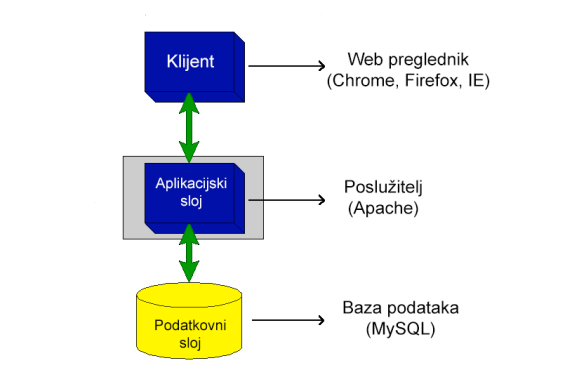
\includegraphics[width=\textwidth]{slike/webAplikacija.png} %veličina slike u odnosu na originalnu datoteku i pozicija slike
			\centering
			\caption{Arhitektura web aplikacije}
			\label{fig:arhitekturaWebApp}
		\end{figure}
		Web aplikacije podijeljene su na tri glavna sloja:
		
		\begin{itemize}
			\item \textbf{Prvi sloj predstavlja prezentacijski sloj}, to je korisničko sučelje i komunikacijski sloj aplikacije gdje korisnik stupa u interakciju s aplikacijom. Glavna svrha prezentacijskog sloja je prikazivanje i prikupljanje informacija od korisnika.
			\item\textbf{Drugi sloj predstavlja aplikacijski sloj}, je glavni sloj web aplikacije. U ovom sloju se informacije prikupljene u prezentacijskom sloju obrađuju korištenjem poslovne logike. Te se također u ovom sloju dohvaćaju unose i izmjenjuju podatci koji se nalaze u podatkovnom sloju
			\item\textbf{Treći sloj je podatkovni sloj}, ili baza podataka je sloj u kojem se pohranjuju podatci koje koristi o obrađuje web aplikacija i u kojem se pristupa istim.
		\end{itemize} 
	
			Svi slojevi međusobno komuniciraju preko standardiziranih Internetskih protokola, kojih se prilikom razvoja 
			aplikacija treba pridržavati.Glavne prednosti razvijanja aplikacija u tri sloja su:
			\begin{itemize}
				\item Svaki sloj može biti napravljen u različitom programskom jeziku i okruženju.
				\item Svaki sloj može biti pokrenut na vlastitom serveru sto znači da slojevi ne ovise jedan o drugom.
				\item Brži razvoj aplikacije zato sto se svaki sloj može razvijati istovremeno.
				\item Poboljšana sigurnost zato sto možemo vršiti provjeru nad upitima i podatcima na tri razine i zbog toga što korisnik ne radi direktno sa SQL serverom.
			\end{itemize}
			Programski jezik kojeg smo odabrali za izradu naše web aplikacije je Java zajedno s Spring Boot-om i Thymeleaf-om. 
			Odabrano razvojno okruženje je IntelliJ IDEA. Arhitektura sustava temeljiti  će se na MVC 
			(Model-View-Controller) konceptu. MVC koncept podržan je od strane Spring Boot radnog okvira i kao takav ima gotove predloške koji nam olakšavaju razvoj web aplikacije.
			MVC koncept sastoji se od:
		\begin{itemize}
			\item \textbf{Model} - Komponenta Model sadrzi cijelu logiku vezanu za podatke s kojom korisnik radi. To mogu biti podatci koji se prenose između komponenti View i Controler ili bilo koje druge podatke vezane za poslovnu logiku.
			\item \textbf{View} - Komponenta View koristi se za svu logiku korisničkog sučelja aplikacije.  Na primjer, korisnički prikaz uključivat će sve komponente korisničkog sučelja kao što su tekstualni okviri, padajući izbornik itd. s kojima je u interakciji krajnji korisnik.
			\item \textbf{Controller} - Kontroleri djeluju kao sučelje između komponenti Modela i Viewa za obradu sve poslovne logike i dolaznih zahtjeva, manipuliranje podacima pomoću komponente Model i interakciju s Viewsima kako bi prikazali konačni izlaz.
		\end{itemize} 
		\eject
			
		\section{Baza podataka}
			

		
			 Arhitekturu dijelimo na tri podsustava:
		\begin{itemize}
			\item 	Web preglednik
			\item 	Poslužitelj
			\item 	Baza podataka	
		\end{itemize}

		\begin{figure}[H]
			
			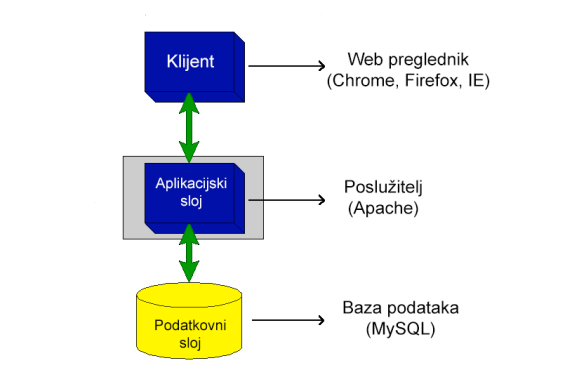
\includegraphics[width=\textwidth]{slike/webAplikacija.png} %veličina slike u odnosu na originalnu datoteku i pozicija slike
			\centering
			\caption{Arhitektura web aplikacije}
			\label{fig:registrirani432132}
		\end{figure}
	
		Princip rada Internet aplikacija temelji se na načinu komunikacije između klijenta i poslužitelja , preko internetske mreže. Zadatak svake Internet aplikacije je prijenos informacija 
		putem Internet protokola od web poslužitelja, do njenog korisničkog sučelja na klijentskoj strani i 
		obrnuto. Na slici 4.1. prikazana je arhitektura Internet aplikacije.

		

			\eject
		\section{Baza podataka}
			
			

			
			
		
		
			\subsection{Opis tablica}
			

				\textit{Svaku tablicu je potrebno opisati po zadanom predlošku. Lijevo se nalazi točno ime varijable u bazi podataka, u sredini se nalazi tip podataka, a desno se nalazi opis varijable. Svjetlozelenom bojom označite primarni ključ. Svjetlo plavom označite strani ključ}
				
				
				\begin{longtblr}[
					label=none,
					entry=none
					]{
						width = \textwidth,
						colspec={|X[6,l]|X[6, l]|X[20, l]|}, 
						rowhead = 1,
					} %definicija širine tablice, širine stupaca, poravnanje i broja redaka naslova tablice
					\hline \multicolumn{3}{|c|}{\textbf{korisnik - ime tablice}}	 \\ \hline[3pt]
					\SetCell{LightGreen}IDKorisnik & INT	&  	Lorem ipsum dolor sit amet, consectetur adipiscing elit, sed do eiusmod  	\\ \hline
					korisnickoIme	& VARCHAR &   	\\ \hline 
					email & VARCHAR &   \\ \hline 
					ime & VARCHAR	&  		\\ \hline 
					\SetCell{LightBlue} primjer	& VARCHAR &   	\\ \hline 
				\end{longtblr}
				
				
			
			\subsection{Dijagram baze podataka}
				
			
			\eject
			
			
		\section{Dijagram razreda}
		
			\textit{Potrebno je priložiti dijagram razreda s pripadajućim opisom. Zbog preglednosti je moguće dijagram razlomiti na više njih, ali moraju biti grupirani prema sličnim razinama apstrakcije i srodnim funkcionalnostima.}\\
			
			\textbf{\textit{dio 1. revizije}}\\
			
			\textit{Prilikom prve predaje projekta, potrebno je priložiti potpuno razrađen dijagram razreda vezan uz \textbf{generičku funkcionalnost} sustava. Ostale funkcionalnosti trebaju biti idejno razrađene u dijagramu sa sljedećim komponentama: nazivi razreda, nazivi metoda i vrste pristupa metodama (npr. javni, zaštićeni), nazivi atributa razreda, veze i odnosi između razreda.}\\
			
			\textbf{\textit{dio 2. revizije}}\\			
			
			\textit{Prilikom druge predaje projekta dijagram razreda i opisi moraju odgovarati stvarnom stanju implementacije}
			
			
			
			\eject
		
		\section{Dijagram stanja}
			
			
			\textbf{\textit{dio 2. revizije}}\\
			
			\textit{Potrebno je priložiti dijagram stanja i opisati ga. Dovoljan je jedan dijagram stanja koji prikazuje \textbf{značajan dio funkcionalnosti} sustava. Na primjer, stanja korisničkog sučelja i tijek korištenja neke ključne funkcionalnosti jesu značajan dio sustava, a registracija i prijava nisu. }
			
			
			\eject 
		
		\section{Dijagram aktivnosti}
			
			\textbf{\textit{dio 2. revizije}}\\
			
			 \textit{Potrebno je priložiti dijagram aktivnosti s pripadajućim opisom. Dijagram aktivnosti treba prikazivati značajan dio sustava.}
			
			\eject
		\section{Dijagram komponenti}
		
			\textbf{\textit{dio 2. revizije}}\\
		
			 \textit{Potrebno je priložiti dijagram komponenti s pripadajućim opisom. Dijagram komponenti treba prikazivati strukturu cijele aplikacije.}